\documentclass[11pt]{article}

\usepackage{physics}
\usepackage[top=1in, bottom=1in, left=0.5in, right=0.5in]{geometry}
\usepackage{hanging}
\usepackage{amsfonts, amsmath, amssymb}
\usepackage[none]{hyphenat}
\usepackage{fancyhdr}
\usepackage[nottoc, notlot, notlof]{tocbibind}
\usepackage{graphicx}
\graphicspath{{./images/}}
\usepackage{float}
\usepackage{siunitx}
\usepackage{esint}

\pagestyle{fancy}
\fancyhead{}
\fancyfoot{}
\fancyhead[L]{MAP2302 Professor Jury}
\fancyhead[R]{Sai Sivakumar 11/23/20}
\fancyfoot[R]{\thepage}
\renewcommand{\headrulewidth}{0pt}

\setlength{\parindent}{0cm}
\setlength{\parskip}{5pt}
\renewcommand{\baselinestretch}{1.25}

\newcommand{\ihat}{\boldsymbol{\hat{\textbf{\i}}}}
\newcommand{\jhat}{\boldsymbol{\hat{\textbf{\j}}}}
\newcommand{\dr}{\vec{r}~^{\prime}(t)}
\newcommand{\dx}{x^{\prime}(t)}
\newcommand{\dy}{y^{\prime}(t)}

\newcommand{\br}[1]{\left(#1\right)}
\newcommand{\sbr}[1]{\left[#1\right]}
\newcommand{\cbr}[1]{\{#1\}}

\newcommand{\dprime}{\prime\prime}

\usepackage{mathtools}

\DeclarePairedDelimiterX{\abr}[1]{\langle}{\rangle}{#1}

\newcommand{\lap}[2]{\mathcal{L}[#1](#2)}

\setcounter{page}{1}

\begin{document}

Section 7.4: 27, 38, Section 7.5: 15, 31, Section 7.6: 19

Section 7.4\\

27. Find $\mathcal{L}^{-1}\{F\}$ for $s^2F(s)-4F(s)=5(s+1)^{-1}$

Rearrange the equation to find $$F(s) = \frac{5}{(s+1)(s-2)(s+2)}$$ which we can expand using the cover-up method into $$F(s) = \frac{-\frac{5}{3}}{s+1} + \frac{\frac{5}{12}}{s-2} + \frac{\frac{5}{4}}{s+2}$$

Using our handy Laplace transforms table the inverse is:
$$-\frac{5}{3}e^{-t} + \frac{5}{12}e^{2t} + \frac{5}{4}e^{-2t}$$

38. First we can give the partial fraction expansion of the rational function like so:
$$\frac{P(s)}{Q(s)} = \frac{A}{s-r} + E(s)$$

The quantity $E(s)$ represents extra terms that are in a form such that each term's denominator is not a multiple of $(s-r)$, since $(s-r)$ is a nonrepeated linear factor of $Q(s)$. Then multiply through by $s-r$ to find:
$$\frac{(s-r)P(s)}{Q(s)}= A + (s-r)E(s)$$

Then take the limit as $s$ tends towards $r$, which immediately causes the extra terms $E(s)$ to vanish:
$$\lim_{s\to r}\frac{(s-r)P(s)}{Q(s)} = A$$

Notice that we may rewrite the left hand side as (using the definition of the derivative):
$$\lim_{s\to r}\frac{1}{\frac{Q(s)-0}{s-r}}P(s) \to \frac{1}{Q^{\prime}(r)}P(r)$$

This is valid so long as the derivative $Q^{\prime}(r)$ is nonzero.

Thus $$A = \frac{P(r)}{Q^{\prime}(s)}$$

Section 7.5\\

15. Use the table along with the initial data:
$$y^{\dprime} - 3y^{\prime}+2y=\cos(t) \to s^2Y(s)+1 -3sY(s) + 2Y(s) = \frac{s}{s^2+1} \to Y(s) = \frac{-(s^2-s+1)}{(s^2+1)(s-1)(s-2)}$$

31. Use the table along with the initial data:
$$y^{\dprime} + 2y^{\prime}+2y=5 \to s^2Y(s)-sa-b + 2sY(s)-2a +2Y(s) = \frac{5}{s} \to Y(s) = \frac{5}{s((s+1)^2+1)}+\frac{a(s+1)+b+a}{(s+1)^2+1}$$

Use the cover-up method to expand part of the first fraction out. Then the following is true, which we can use to deduce the other fraction (whose numerator is $Bs+C$):
$$5 = \frac{5}{2}((s+1)^2+1) + Bs^2+Cs \implies B=-\frac{5}{2}, C=-5$$
$$\to Y(s) = \frac{\frac{5}{2}}{s} + \frac{-\frac{5}{2}s-5}{(s+1)^2+1}+\frac{a(s+1)+b+a}{(s+1)^2+1}$$
$$\to y(t) = \frac{5}{2}  -\frac{5}{2}e^{-t}\sin(t) -\frac{5}{2}e^{-t}\cos(t) + ae^{-t}\cos(t) + be^{-t}\sin(t)+ ae^{-t}\sin(t)$$
$$\to y(t) = \frac{5}{2} + \br{a-\frac{5}{2}}e^{-t}\cos(t) + \br{a+b-\frac{5}{2}}e^{-t}\sin(t)$$

Section 7.6\\

19. First give $g(t) = 20-\Pi_{3\pi,4\pi}(t)$. I will call the Laplace transform of $I(t)$ as $Y(s)$ just because a capital letter was already in use. Apply the Laplace transform to both sides:
$$I^{\dprime}(t) + 2I^{\prime}(t)+2I = g(t) \to s^2Y(s)-10s + 2sY(s)-20 +2Y(s) = \frac{20}{s} - e^{-3\pi s}\frac{20}{s} + e^{-4\pi s}\frac{20}{s}$$
$$\to Y(s) = 20\br{1-e^{-3\pi s}+e^{-4\pi s}}\br{\frac{1}{s(\br{s+1}^2+1)}}  + \frac{10(s+1) + 10}{\br{s+1}^2+1}$$
$$\to Y(s) = 20\br{1-e^{-3\pi s}+e^{-4\pi s}}\br{\frac{\frac{1}{2}}{s}+\frac{-\frac{1}{2}s-1}{\br{s+1}^2+1}} + \frac{10(s+1) + 10}{\br{s+1}^2+1} \text{ using a similar process as \#31}$$
$$\to I(t) = 20\br{\frac{1}{2}-\frac{1}{2}e^{-t}\sin(t)-\frac{1}{2}e^{-t}\cos(t)}-20u(t-3\pi)\br{\frac{1}{2}-\frac{1}{2}e^{-(t-3\pi)}\sin(t-3\pi)-\frac{1}{2}e^{-(t-3\pi)}\cos(t-3\pi)}$$
$$+20u(t-4\pi)\br{\frac{1}{2}-\frac{1}{2}e^{-(t-4\pi)}\sin(t-4\pi)-\frac{1}{2}e^{-(t-4\pi)}\cos(t-4\pi)}+ 10\br{e^{-t}\sin(t)+e^{-t}\cos(t)}$$
$$\to I(t) = 10-10u(t-3\pi)\br{1+e^{-(t-3\pi)}\sin(t) + e^{-(t-3\pi)}\cos(t)}+10u(t-4\pi)\br{1-e^{-(t-4\pi)}\sin(t) - e^{-(t-4\pi)}\cos(t)}$$
\newpage
A sketch of the current looks like:

\begin{figure}[h]
    \centering
    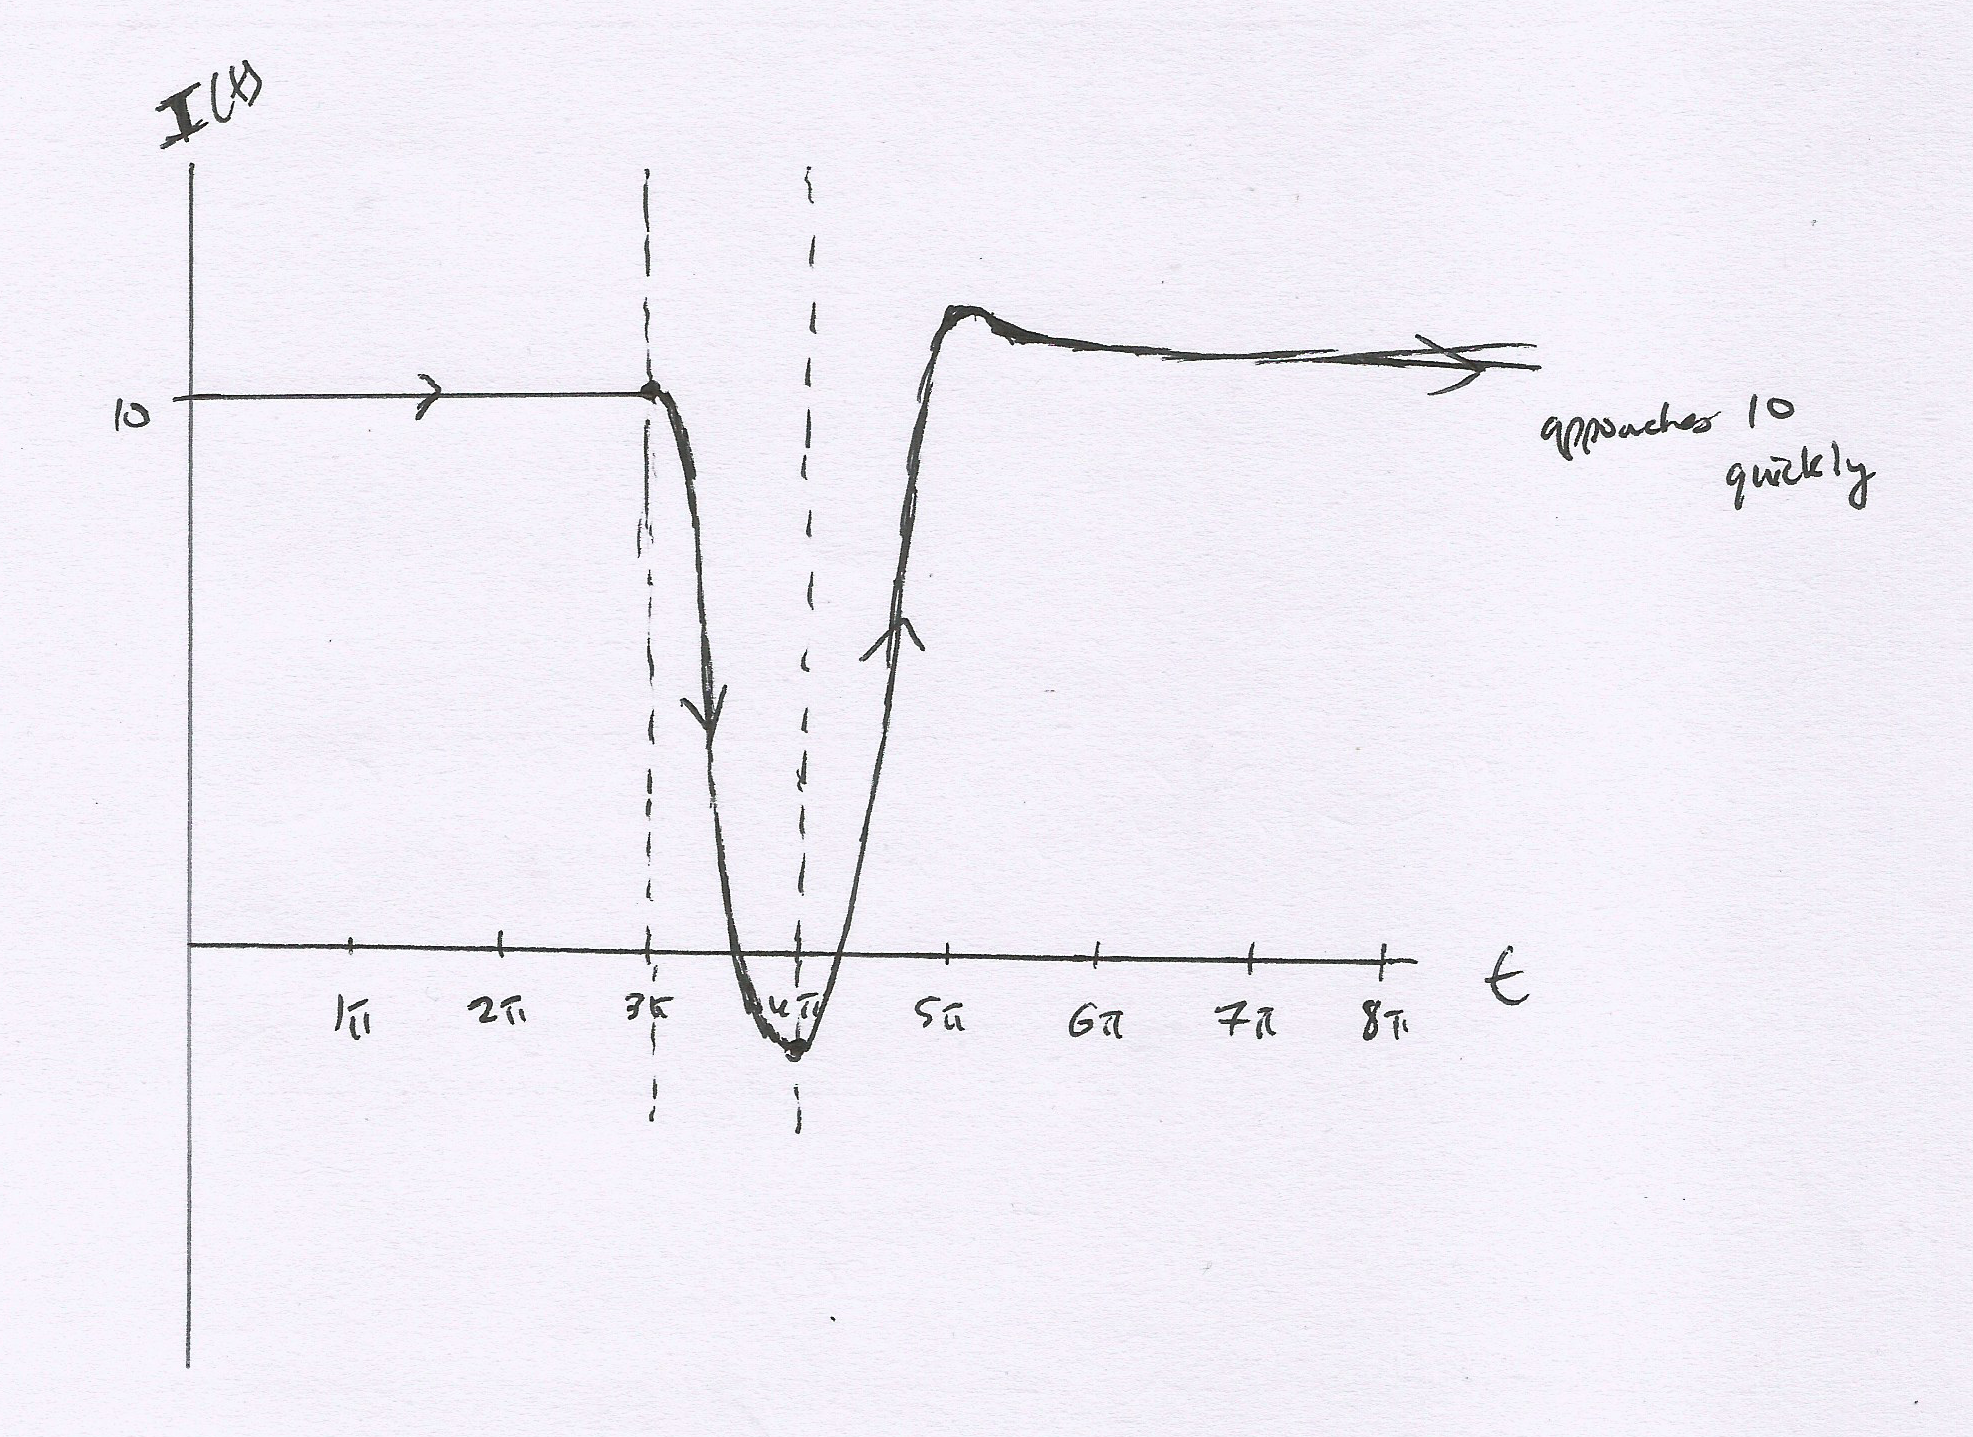
\includegraphics[scale=0.75]{sketch}
\end{figure}

\end{document}